\documentclass[a4paper]{article}

%% Language and font encodings
\usepackage[french]{babel}
\usepackage[utf8x]{inputenc}
\usepackage[T1]{fontenc}

%% Sets page size and margins
\usepackage[a4paper,top=3cm,bottom=3cm,left=2cm,right=2cm,marginparwidth=2cm]{geometry}

%% Useful packages
\usepackage{amsmath}
\usepackage{graphicx}
\usepackage[colorinlistoftodos]{todonotes}
\PassOptionsToPackage{hyphens}{url}
\usepackage[colorlinks=true, allcolors=black]{hyperref}
\usepackage{fourier-orns}
\usepackage{titlesec}
\usepackage{fancyhdr}
\usepackage{fancyvrb}
\pagestyle{fancy} 
\setcounter{tocdepth}{5}
\usepackage{fancyvrb}

%% Pour les exemples
\usepackage{mdframed}
\newmdenv[topline=false, bottomline=false, rightline=false, skipabove=\topsep, skipbelow=\topsep]{example}

\usepackage{libertine}
\newcommand{\hsp}{\hspace{20pt}}
\newcommand{\HRule}{\rule{\linewidth}{0.5mm}}

\renewcommand{\headrulewidth}{1pt}
\fancyhead[C]{} 
\fancyhead[L]{}
\fancyhead[R]{\footnotesize{\leftmark}}

\renewcommand{\footrulewidth}{1pt}
\fancyfoot[C]{} 
\fancyhead[L]{}
\fancyfoot[R]{\thepage}

\definecolor{Zgris}{rgb}{0.87,0.85,0.85}

\usepackage{eso-pic,graphicx}
\usepackage{xcolor}
\newcommand{\bgimg}[1] {
    \AddToShipoutPicture {
        \put(\LenToUnit{0 cm},\LenToUnit{0 cm}) {
            \includegraphics[width=\paperwidth,height=\paperheight]{#1}
        }
    }
}

%% To list and caption code
\usepackage{minted}
\renewcommand{\listoflistingscaption}{Table des programmes}
\usepackage{caption}
\newenvironment{code}{\captionsetup{type=listing}}{}
\renewcommand{\listingscaption}{Programme}
\renewcommand{\arraystretch}{1.2} %% row 20% longer

\begin{document}




\begin{titlepage}
    \begin{sffamily}
        \begin{center}

            
\includegraphics[width=5cm]{images/LogoHenallux.PNG}~\\[1.5cm]
            \textsc{\Large Rapport de laboratoire}\\[1.5cm]

            \HRule \\[0.4cm]
            { \huge \bfseries Manipulation 3 : Mémoire volatile\\[0.4cm] }
            \HRule \\[2cm]

            \begin{minipage}{0.4\textwidth}
                \begin{flushleft} \large
                    Roumache Grégoire\\
                    Sénéchal Julien\\
                    Wallemme Maxime\\
                \end{flushleft}
            \end{minipage}
            \begin{minipage}{0.55\textwidth}
                \begin{flushright} \large
                    IR317 - Forensics and cyberattack evidence 2021-2022\\
                    Sécurité des systèmes, Hénallux\\
                    Troisième année, Classe A Groupe 1 \\
                \end{flushright}
            \end{minipage}
            \vfill

            {\large 28 Décembre 2021}

        \end{center}
    \end{sffamily}
\end{titlepage}

\let\cleardoublepage\clearpage










\tableofcontents \newpage










\section{Introduction}

Dans le cadre de ce laboratoire, nous avons analysé la mémoire volatile de l'ordinateur potentiellement infecté du CHR. Nous avons utilisé les outils Volatility 2 (version 2.6) ainsi que Volatility 3 (version 1.0.0). Ce sont des outils d'analyse Forensics permettant d'aller chercher certaines informations précises contenues dans la mémoire volatile capturée. Notre but était de récolter des preuves pouvant aider à confirmer nos hypothèses concernant l'implantation d'un malware sur le PC de l'hôpital par notre suspect.










\section{Analyse de la mémoire volatile}

Nous avons pu obtenir les différents processus lancés ainsi que leur PID et les arguments utilisés pour lancer le processus en ligne de commande à l'aide de la commande suivante:
\begin{example}
    vol.py -{}-profile=Win10x64\_19041 cmdline -f file.dmp
\end{example}
Parmi ces résultats, deux d'entre eux pouvaient potentiellement mener à des preuves supplémentaires:
\begin{center}
    \begin{tabular}{lll} \hline
        \textbf{Nom} & \textbf{PID} & \textbf{Ligne de commande} \\ \hline
        python2.exe  & 7960         & \texttt{\small python2 xenotix\_python\_logger.py local} \\
        python.exe   & 6832         & \texttt{\small python3 client.py} \\ \hline
    \end{tabular}
\end{center}

Nous pouvons également observer sur la figure \ref{fig:process-utilisateur} que ce sont les seuls processus suspects venant de \textit{explorer.exe} duquel découlent tout les processus lancés par l'utilisateur. Ces résultats ont été obtenus avec cette commande:
\begin{example}
    vol.py -{}-profile=Win10x64\_19041 pstree -f file.dmp
\end{example}

\begin{figure}[H]
    \centering
    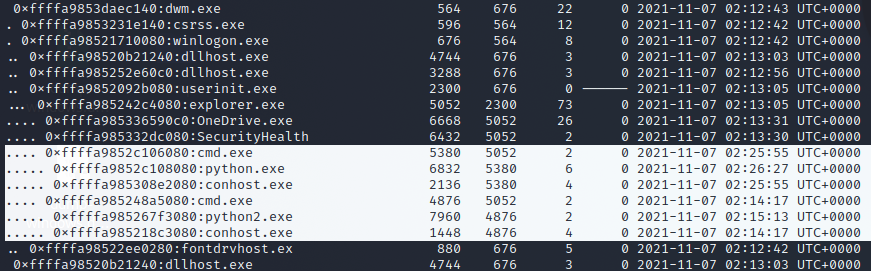
\includegraphics[width=0.85\linewidth]{images/02-process-utilisateur.png}
    \caption{Arbres des processus}
    \label{fig:process-utilisateur}
\end{figure}

Les lignes de commandes ayant lancés ces deux processus utilisent chacune un script python qu'il est intéressant de récupérer parce qu'ils pourraient potentiellement être retrouvés sur la clé USB du suspect. Afin de tester cette hypothèse, nous devons réaliser un dump de la mémoire de chacun de ces processus et l'analyser ensuite. Pour ce faire, nous avons utilisé la commande suivante:
\begin{example}
    vol.py -f “/path/to/file” ‑{}‑profile <profile> procdump -p <PID> ‑{}‑dump-dir=“/path/to/dir”
\end{example}

Elle permet d'obtenir un dump d'un processus et nous l'avons donc exécutée à deux reprises, pour les processus de PID 7960 et PID 6832. Dans ces derniers, nous avons pu obtenir les codes sources des scripts utilisés. Ainsi, vous pouvez voir le script \textit{xenotix\_python\_logger.py} sur la figure \ref{fig:github-keylogger} retrouvé dans le dump du processus 7960. Ce fichier contient également un lien vers le répertoire GitHub dont il est issu, c'est-à-dire: {\small \url{https://github.com/ajinabraham/Xenotix-Python-Keylogger}}.

Sur la figure \ref{fig:ip-rootkit}, nous retrouvons le fichier python \textit{client.py}. Nous avons réussi à trouver sa provenance. En effet, ce programme n'a pas été écrit spécifiquement pour cette attaque mais il a été copié du répertoire GitHub suivant: {\small \url{https://github.com/TOG6-6/MULTI-PC-VIRUS/blob/main/door.py}}, et l'adresse IP a été modifiée. Cependant, nous n'avons pas trouvé cette adresse IP (5.135.163.141) dans nos investigations précédentes et elle demandera de plus amples recherches.

\begin{figure}[H]
    \centering
    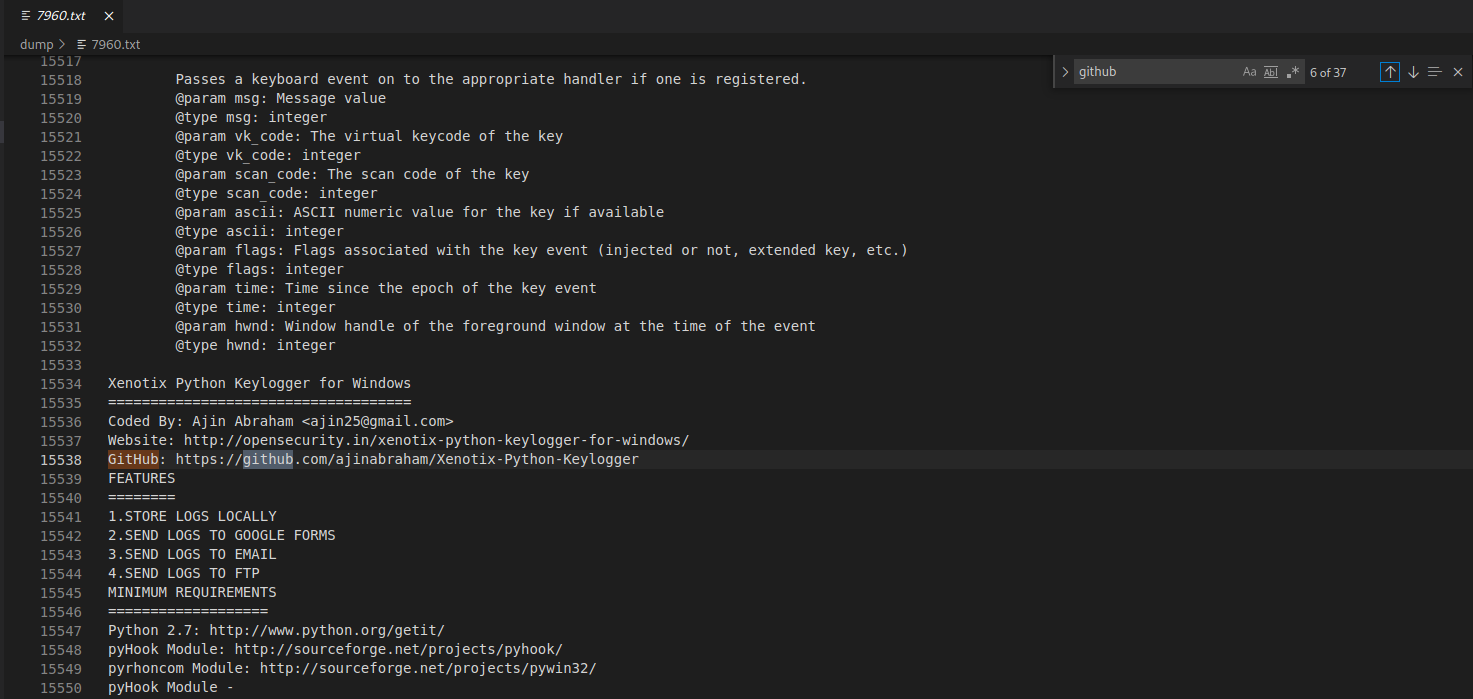
\includegraphics[width=0.89\linewidth]{images/04-github-keylogger.png}
    \caption{Chaîne de caractères du processus 7960 indiquant le répertoire GitHub \textit{Xenotix-Python-Keylogger}}
    \label{fig:github-keylogger}
\end{figure}

\begin{figure}[H]
    \centering
    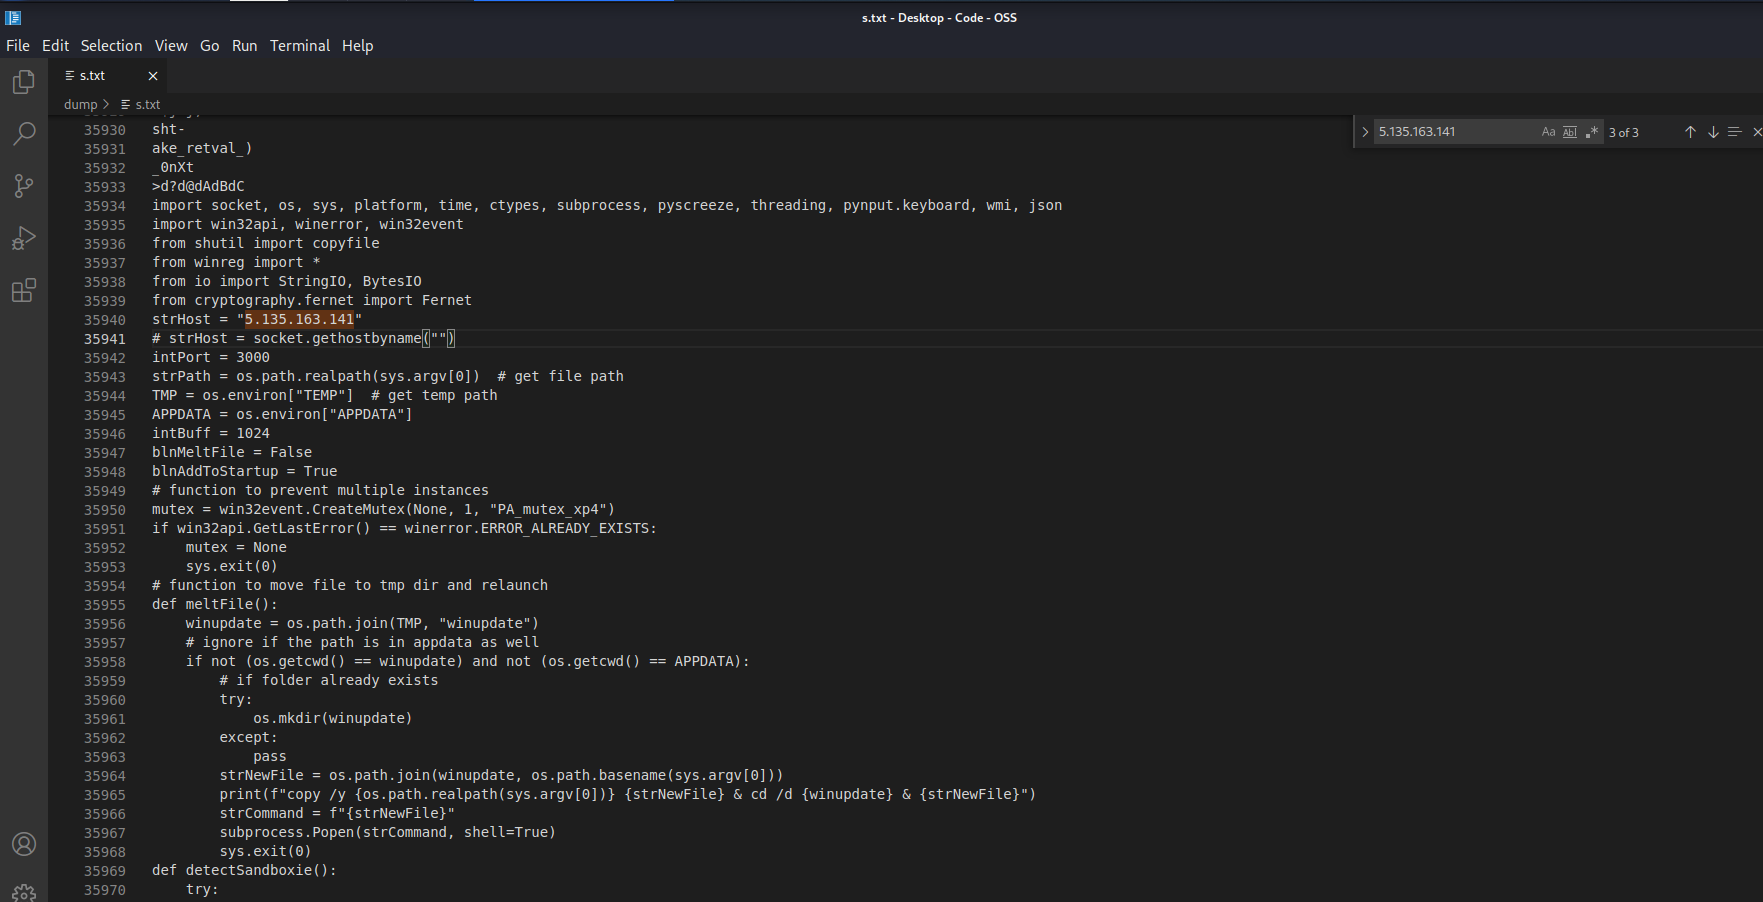
\includegraphics[width=0.89\linewidth]{images/05-ip-suspecte-rootkit.png}
    \caption{Backdoor python \textit{client.py} retrouvée dans le processus 6832}
    \label{fig:ip-rootkit}
\end{figure}

Lors de l'analyse des dumps mémoires, nous avons également remarqué une chaîne de caractères très intéressante. Celle-ci est mise en évidence sur la figure \ref{fig:github-rootkit}, c'est un indice montrant que le système a pu être infecté par le rootkit r77 \cite{3}. Ce malware est particulier parce qu'il ne laisse aucune trace sur le système de fichiers de la machine infectée, cependant, il écrit son exécutable dans une clé de registre Windows. Nous pouvons donc confirmer sa présence en les listant, ce que nous pouvons faire avec cette commande:
\begin{example}
    python3 vol.py -f ../dump-windows.dump windows.registry.printkey.PrintKey | grep $\backslash$\$77
\end{example}
Ce qui nous donne le résultat suivant:
\begin{example}
\begin{Verbatim}[fontsize=\footnotesize]
0xc108ceacd000 inKeyed    \SystemRoot\System32\Config\SOFTWARE $77config False
0xc108ceacd000 REG_BINARY \SystemRoot\System32\Config\SOFTWARE $77stager False
\end{Verbatim}
\end{example}
Montrant donc que cette ordinateur est bien infecté par ce malware qui est stocké dans le registre \textit{\$77stager}, et dont la configuration se situe dans le registre \textit{\$77config}, tous les deux situés à cet emplacement: \\
\textit{$\backslash$SystemRoot$\backslash$System32$\backslash$Config$\backslash$SOFTWARE$\backslash$}.

\begin{figure}[H]
    \centering
    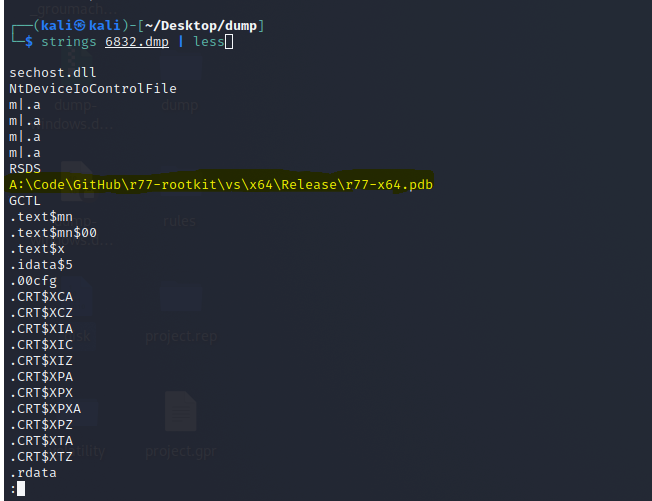
\includegraphics[width=0.75\linewidth]{images/03-github-rootkit.png}
    \caption{Chaîne de caractères du processus 6832 indiquant le répertoire GitHub \textit{r77-rootkit}}
    \label{fig:github-rootkit}
\end{figure}

Nous tentons ensuite volatility avec les arguments suivants entrés en commande:
\begin{itemize}
    \item filescan
    \item mftparser\\
\end{itemize}
Nous avons pu obtenir des informations concernant la présence et la localisation du malware keylogger sur la machine de l'hôpital. À l'aide de l'argument \textit{filescan}, nous avons pu obtenir l'information sur la présence d'un fichier caché sur le bureau du compte utilisateur \textit{Infirmier}. Ce dernier contenait un dossier nommé \textit{keylog}.

\begin{figure}[H]
    \centering
    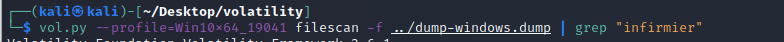
\includegraphics[width=14cm]{images/Commande_filescan_User_infirmier.png}
    \caption{Commande filescan utilisée}
    \label{fig:filescan_command}
\end{figure}

\begin{figure}[H]
    \centering
    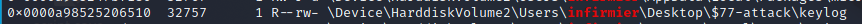
\includegraphics[width=15cm]{images/Dossier_user _infirmier.png}
    \caption{Dossier caché trouvé sur le bureau de l'utilisateur}
    \label{fig:dossier_user_infirmier}
\end{figure}

Ensuite, avec l'argument \textit{mftparser}, nous avons pu obtenir le nom des fichiers présents dans le dossier caché \textit{keylog} du bureau de l'utilisateur infirmier.
Parmi ceux-ci, se trouvait le fichier \textit{xenotix\_python\_logger.py}

\begin{figure}[H]
    \centering
    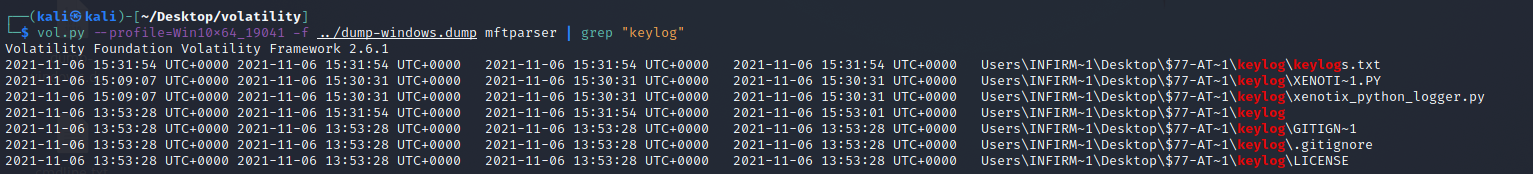
\includegraphics[width=0.99\linewidth]{images/keylog.png}
    \caption{Contenu du dossier caché Keylog}
    \label{fig:contenu_keylog}
\end{figure}














\newpage
\section{Correspondances entre les différentes analyses réalisées}

Sur la figure \ref{fig:keylogger_usb}, nous pouvons observer que le script \emph{xenotix\_python\_logger.py} se trouvait également sur la clé USB de la première analyse. Ce qui nous donne des raisons de penser que le script à bien été mis en place suite à cette attaque et que celui-ci n'est donc pas issu d'une attaque antérieure.\\
Il en va de même pour le script \emph{client.py} que l'on peu retrouver également sur la figure \ref{fig:client_usb}.

\begin{figure}[H]
    \centering
    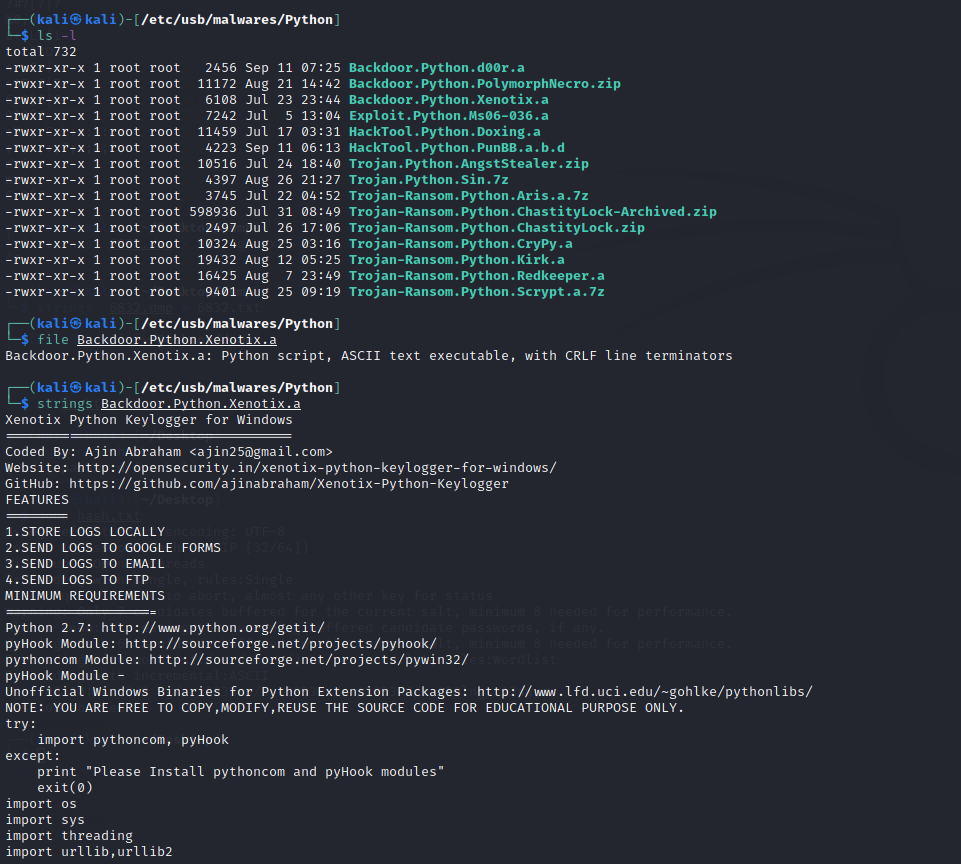
\includegraphics[width=0.99\linewidth]{images/keylogger_usb.png}
    \caption{Code source du Keylogger sur la clé USB}
    \label{fig:keylogger_usb}
\end{figure}

\begin{figure}[H]
    \centering
    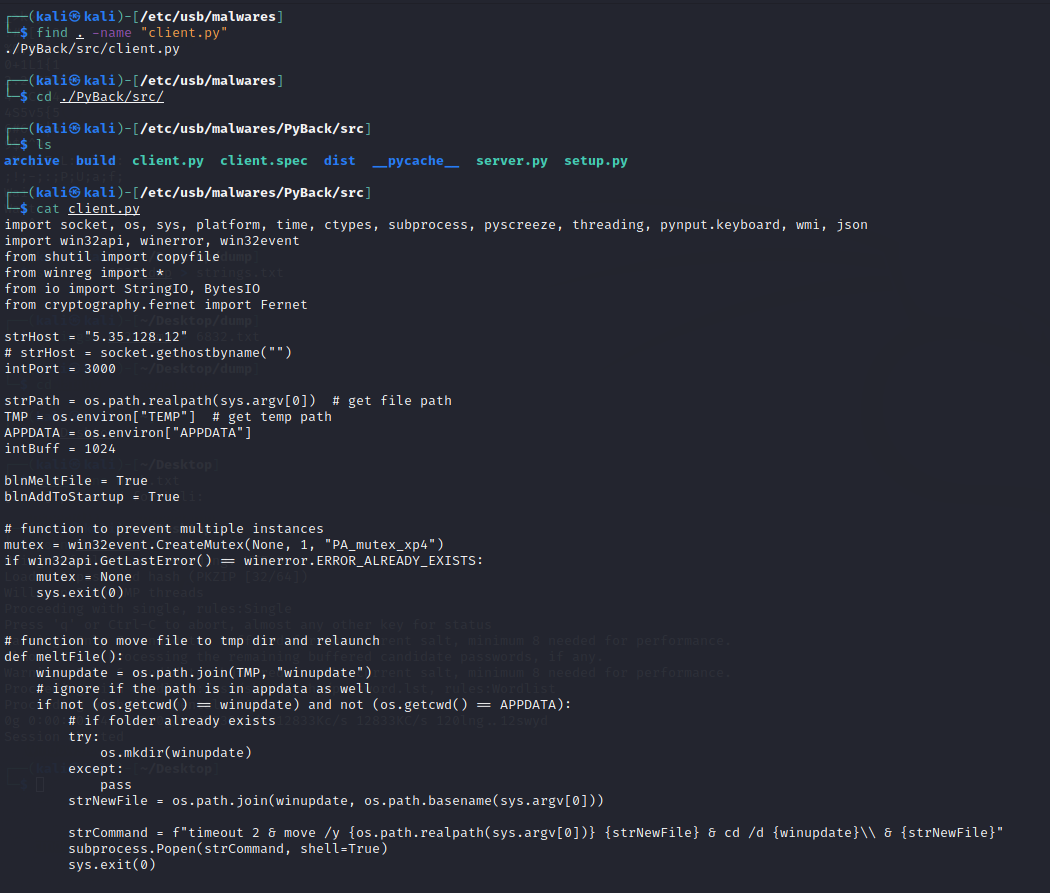
\includegraphics[width=0.99\linewidth]{images/client.py_usb.png}
    \caption{Code source de la backdoor sur la clé USB}
    \label{fig:client_usb}
\end{figure}










\section{Conclusion}

Tout d'abord, lors de cette analyse nous avons pu établir divers liens entre les analyses effectuées dans le cadre de cette enquête. En effet, nous avons pu remarquer la présence de scripts retrouvés sur la clé USB laissée tomber au CHR par le présumé attaquant. Ces mêmes scripts contenaient une adresse IP qu'il serait intéressant de rechercher afin d'avancer un peu plus loin dans l'enquête. Ensuite, nous avons pu déterminer quels scripts malveillants étaient cachés sur la machine à l'aide d'un rootkit et comment celui-ci fonctionnait pour procéder à la dissimulation de ceux-ci. Enfin, nous avons retrouvé les dossiers et fichiers ajoutés par le keylogger sur la machine du CHR.










\newpage \appendix

\section{Analyse du dump de la mémoire sous Windows}



\subsection{Volatility 2}

Tout d'abord, nous avons voulu analyser le dump mémoire que nous avions réalisé à l'aide de l'outil FTKImager (version 3.2.0) avec Volatility2 (version 2.6). Mais après avoir utilisé la commande suivante:
\begin{example}
    vol2.exe -f FILE imageinfo
\end{example}
qui nous a permis de trouver le profil à utiliser pour les autres commandes. Nous avons réalisé que la version de Windows sur laquelle nous avions effectué le dump mémoire était trop récente. Volatility2 ne prenait pas en charge cette version et il n'existait donc pas de profil correspondant. Nous avons donc utilisé Volatility3 pour réaliser l'analyse.



\subsection{Volatility 3}

Nous avons utilisé l'outil Volatility3 (version 1.0.0) afin de réaliser l'analyse du dump mémoire de Windows. Les commandes utilisées nous ont permis de récolter différentes informations intéressantes et d'apprendre à utiliser l'outil d'analyse pour la suite de la manipulation. A chaque commande, nous avons rediriger la sortie de la commande vers un fichier texte afin de conserver les informations recueillies et de pouvoir les analyser plus facilement.

Commandes et résultats:
\begin{enumerate}
    \item python vol.py -f memdump.mem windows.cmdline.CmdLine > CmdHistory.txt
    \begin{itemize}
        \item L'option \textit{-f} permet de spécifier le fichier à analyser
        \item \textit{windows.cmdline.CmdLine} sert à obtenir l'historique des commandes utilisées dans l'outil CMD lors de la capture de la mémoire
    \end{itemize}
    \begin{figure}[H]
        \centering
        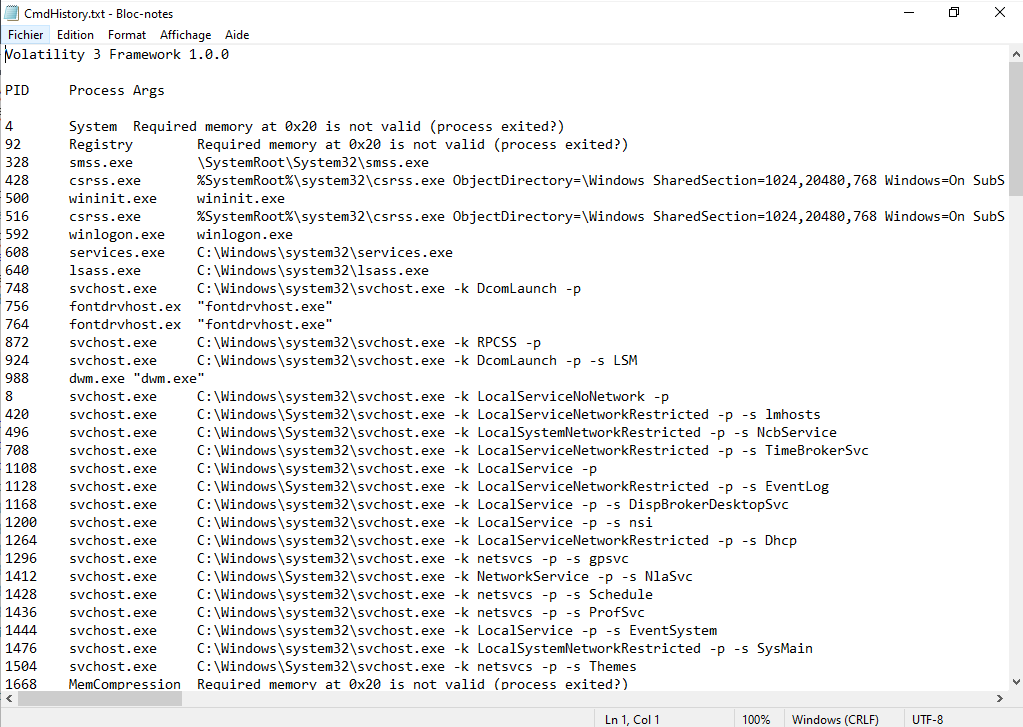
\includegraphics[width=15cm]{images/CmdHistory.png}
        \caption{Résultat de la commande - Historique CMD}
        \label{cmdhistory}
    \end{figure}
    \item python vol.py -f memdump.mem windows.netscan.NetScan > NetworkInfo.txt
    \begin{itemize}
        \item \textit{windows.netscan.NetScan} permet de récupérer les informations sur le réseau
    \end{itemize}
    \begin{figure}[H]
        \centering
        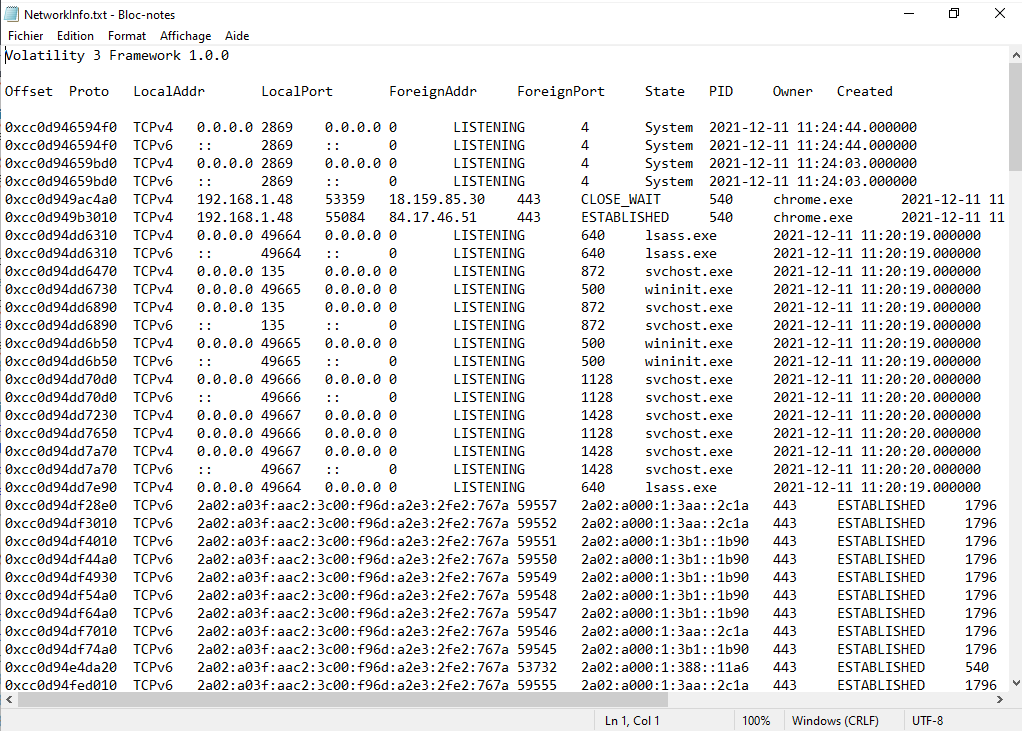
\includegraphics[width=15cm]{images/NetworkInfo.png}
        \caption{Résultat de la commande - Informations sur le réseau}
        \label{networkinfo}
    \end{figure}
    \item python vol.py -f memdump.mem windows.pslist.PsList > ProcessList.txt
    \begin{itemize}
        \item \textit{windows.pslist.PsList} sert à récupérer une liste des processus en cours d'exécution lors de la capture de la mémoire
    \end{itemize}
    \begin{figure}[H]
        \centering
        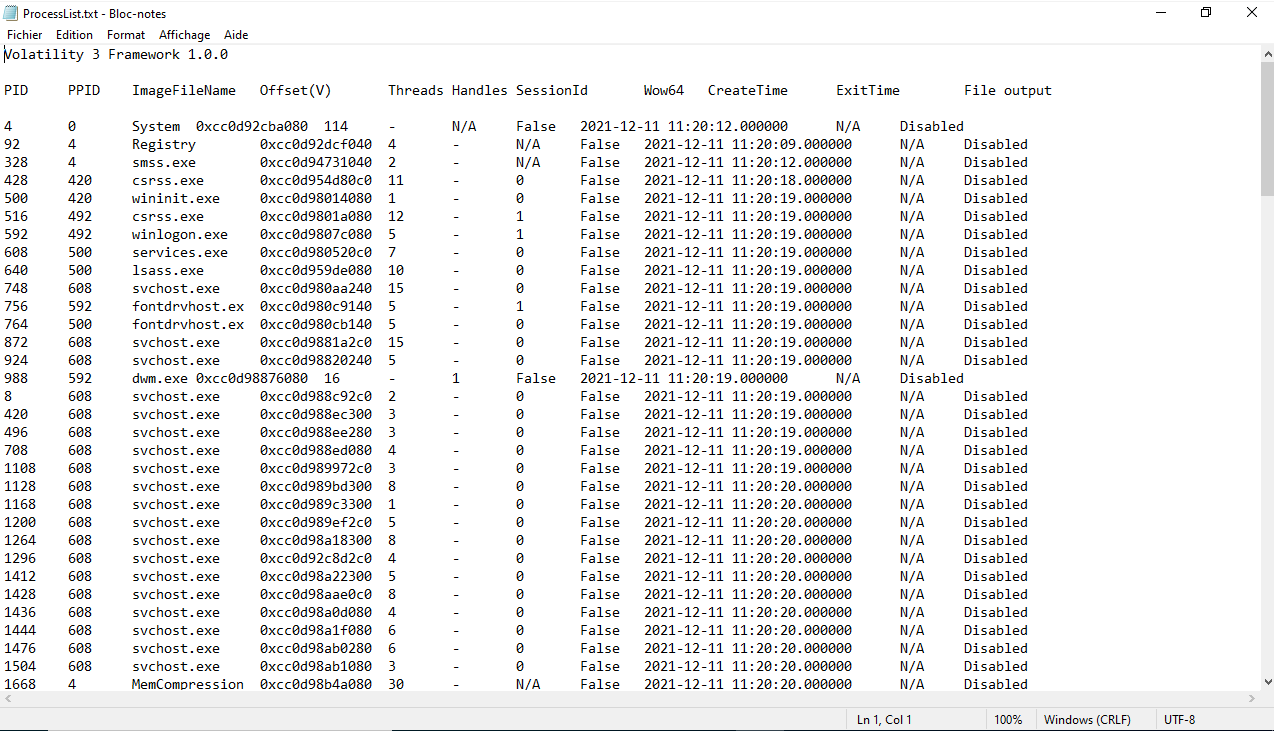
\includegraphics[width=15cm]{images/ProcessList.png}
        \caption{Résultat de la commande - Liste des processus en cours d'exécution}
        \label{processlist}
    \end{figure}
    \item python vol.py -f memdump.mem windows.psscan.PsScan > HiddenProcess.txt
    \begin{itemize}
        \item \textit{windows.psscan.PsScan} permet de retrouver les processus cachés en cours d'exécution lors de la capture de la mémoire
    \end{itemize}
    \begin{figure}[H]
        \centering
        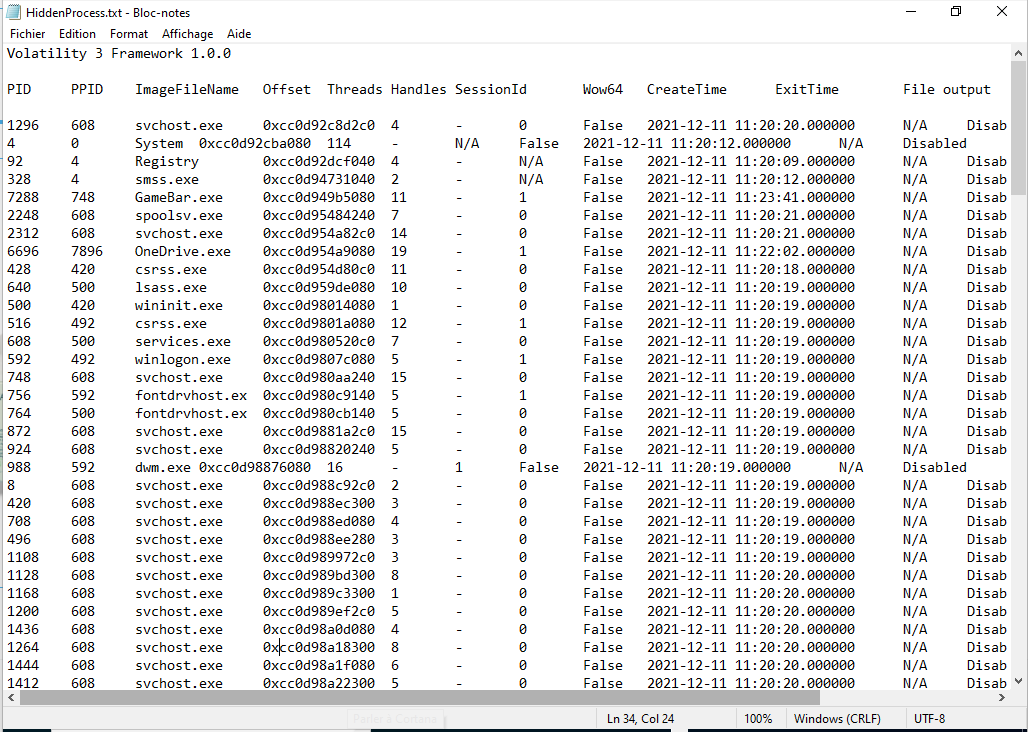
\includegraphics[width=15cm]{images/HiddenProcess.png}
        \caption{Résultat de la commande - Processus cachés}
        \label{hiddenprocess}
    \end{figure}
    \item python vol.py -f memdump.mem windows.getservicesids.GetServiceSIDs > ServiceList.txt
    \begin{itemize}
        \item \textit{windows.getservicesids.GetServiceSIDs} permet de lister les services en cours d'exécution lors de la capture de la mémoire
    \end{itemize}
    \begin{figure}[H]
        \centering
        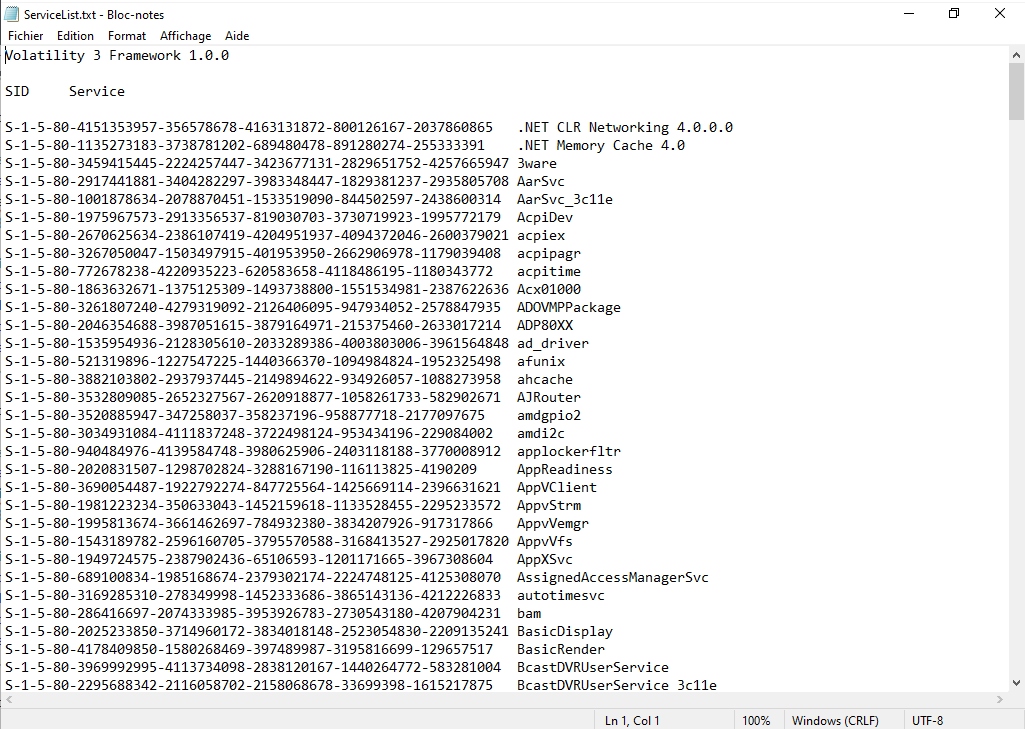
\includegraphics[width=15cm]{images/ServiceList.png}
        \caption{Résultat de la commande - Listes des services}
        \label{servicelist}
    \end{figure}
    \item python vol.py -f memdump.mem windows.driverscan.DriverScan > DriverScan.txt
    \begin{itemize}
        \item \textit{windows.driverscan.DriverScan}
    \end{itemize}
    \begin{figure}[H]
        \centering
        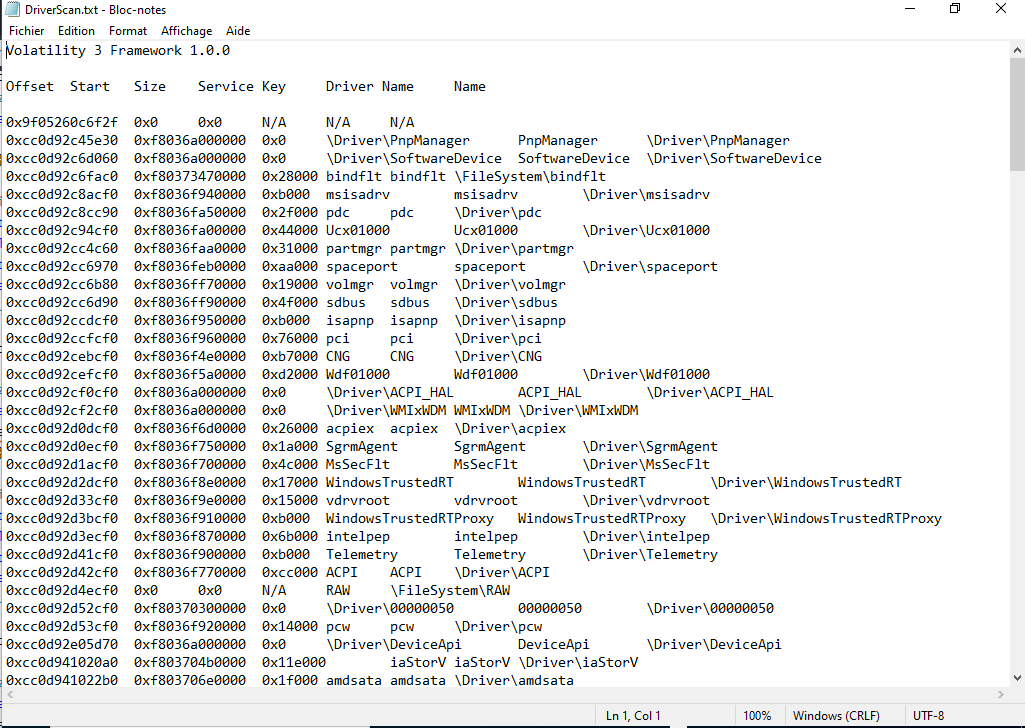
\includegraphics[width=15cm]{images/DriversList.png}
        \caption{Résultat de la commande - Listes des Drivers}
        \label{driverslist}
    \end{figure}
    Nous aurions voulu récupérer le texte entré dans l'outil notepad ainsi que l'historique web mais ces fonctionnalités ne sont pas disponible avec l'outil Volatility3.
\end{enumerate}

\section{Analyse du dump de la mémoire sous Linux}
\subsection{Lime}
Afin de procéder à la manipulation, il est tout d'abord nécessaire de procéder à l'installation/mise à jour de plusieurs paquets :
\begin{itemize}
    \item linux-headers-\$(uname -r)
    \item lime-forensics-dkms
    \item mlocate
\end{itemize}
Ensuite, il sera plus simple d'actualiser la base de donnée de \emph{locate}.
Enfin, il nous suffire de faire la commande suivante afin d'obtenir un dump de la mémoire (voir figure \ref{fig:captureLinux}) :
\begin{example}
    insmod \$(locate lime.ko | head -n 1) "path=<\emph{Nom du fichier de sortie}> format=lime"
\end{example}
\begin{figure}[H]
    \centering
    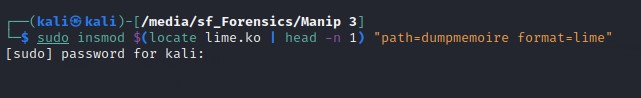
\includegraphics[width=0.99\textwidth]{images/linux/1.jpg}
    \caption{Capture de la mémoire sous Linux}
    \label{fig:captureLinux}
\end{figure}

\subsection{Volatility 2}
Beaucoup plus de plugins et d'options sont disponibles pour Linux sur volatility 2. Malheureusement, nous avons heurté un problème lors de la création d'un profil correspondant à notre machine de test. Nous n'avons donc pas eu la possibilité d'analyser notre mémoire grâce à volatility 2. Notre analyse de cette image sera malheureusement donc beaucoup moins poussé car elle se fera exclusivement sur volatility 3.

\subsection{Volatility 3}

Afin de pouvoir utiliser volatility 3, il sera tout d'abord nécessaire de générer une table des symboles afin de permettre l'interprétation du dump mémoire. Il s'agit d'une étape qui n'est pas nécessaire pour les dumps provenant d'une machine Windows. Ceci est dû à la diversité des noyaux Linux/Mac.\\\\

Une fois cela fait, nous pouvons tout d'abord commencer notre analyse en listant les différents processus :
\begin{example}
    vol -f dumpmemoire linux.pslist > ListProcs
\end{example}

Nous pouvons remarquer qu'un processus \emph{nano} était lancé avec le PID 1507 (voir figure \ref{fig:nano}). Il peut-être intéressant de récupérer la mémoire liée à ce PID afin de voir quel fichier était modifié/créé et voir ainsi le contenu de celui-ci. Malheureusement, volatility 3 étant encore à la version 1.0.0, celui-ci ne propose pas encore de solutions afin de récupérer la mémoire d'un processus sous Linux (ce qui n'est pas le cas des machines Windows par exemple).

\begin{figure}[H]
    \centering
    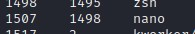
\includegraphics[width=0.49\textwidth]{images/linux/3.jpg}
    \caption{Processus nano dans la liste des processus}
    \label{fig:nano}
\end{figure}

Il peut parfois être intéressant d'utiliser le plugin \emph{pstree}. Celui va permettre de lister également les processus lancés mais aussi de les trier selon leur arborescence.
\begin{example}
    vol -f dumpmemoire linux.pstree > TreeProcs
\end{example}

Sur la figure \ref{fig:pstree}, on peut voir un exemple de l'arborescence partant de \emph{systemd} jusque \emph{nano}.

\begin{figure}[H]
    \centering
    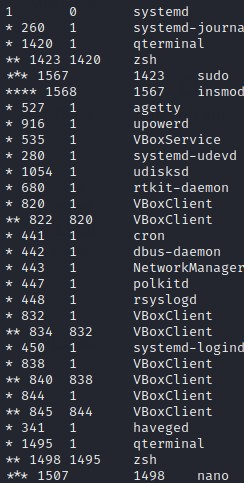
\includegraphics[width=0.25\textwidth]{images/linux/5.jpg}
    \caption{Arborescence des processus jusque nano}
    \label{fig:pstree}
\end{figure}

Il est également possible d'énumérer un certain nombre d'appels systèmes qui ont été mémorisés depuis le lancement de la machine.
\begin{example}
    vol -f dumpmemoire linux.check\_syscall.Check\_syscall > syscall
\end{example}

La sortie possède 5 colonnes :
\begin{itemize}
    \item La table des adresses
    \item Les noms
    \item L'index
    \item Le gestionnaire d'adresses
    \item Le gestionnaire de symboles\\\\
\end{itemize}

Un autre plugin, permet de lister les différents shells tty ouvert lors de la capture (voir figure \ref{fig:tty}).

\begin{example}
    vol -f dumpmemoire linux.tty\_check.tty\_check > ttylist
\end{example}

\begin{figure}[H]
    \centering
    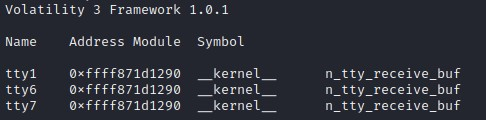
\includegraphics[width=0.70\textwidth]{images/linux/9.jpg}
    \caption{Liste des shells tty ouvert}
    \label{fig:tty}
\end{figure}

Comme dit précédemment, il n'est pas possible d'extraire la mémoire d'un processus sous Linux avec volatility 3. Néanmoins, il nous est possible de faire une carte mémoire. La figure \ref{fig:mapnano} nous montre la carte mémoire de nano (pid 1507).

\begin{example}
    vol -f dumpmemoire linux.proc.Maps --pid <pid> > map
\end{example}

\begin{figure}[H]
    \centering
    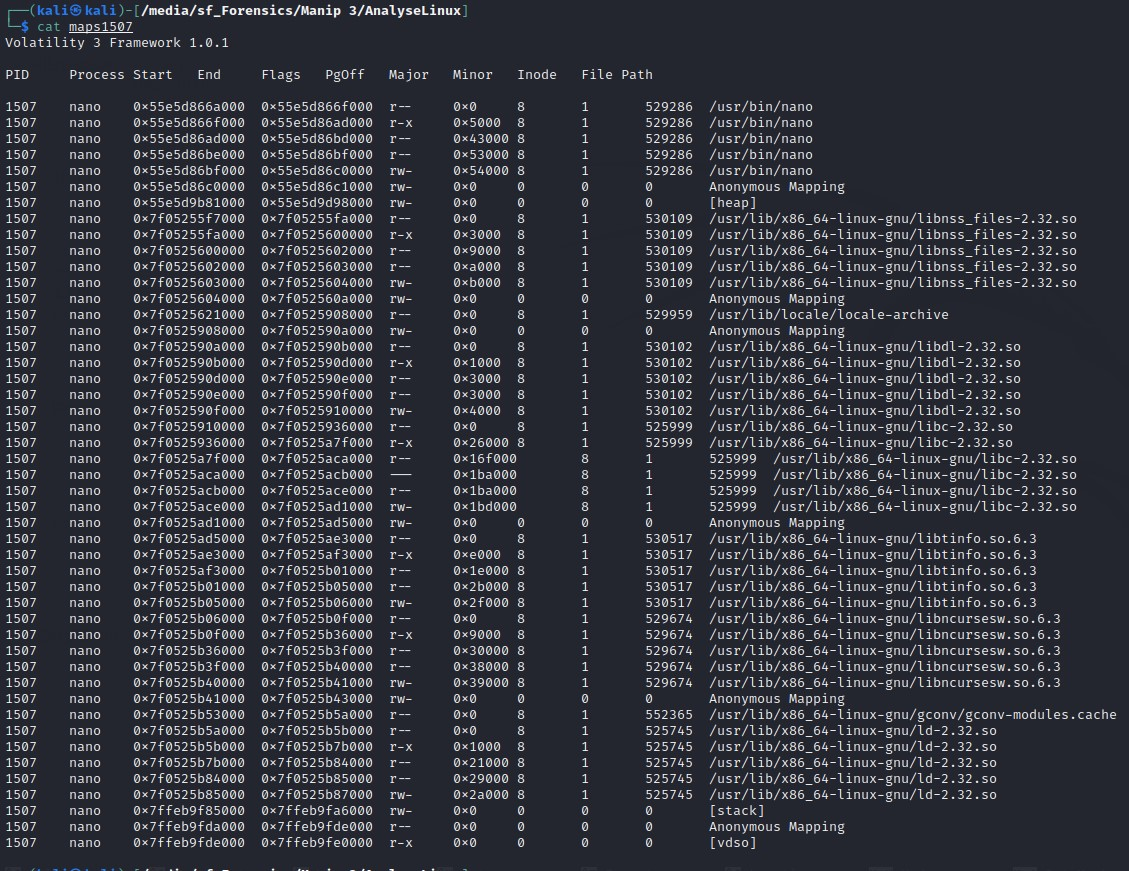
\includegraphics[width=0.70\textwidth]{images/linux/11.jpg}
    \caption{Carte mémoire de nano}
    \label{fig:mapnano}
\end{figure}














\newpage \addcontentsline{toc}{section}{Table des figures} \listoffigures
\newpage \addcontentsline{toc}{section}{Références}
\begin{thebibliography}{9}
\bibitem{1} consulté le 12-12-2021, {\footnotesize \url{https://book.hacktricks.xyz/forensics/basic-forensic-methodology/memory-dump-analysis/volatility-examples}}
\bibitem{2} consulté le 20-12-2021, {\footnotesize \url{https://blog.onfvp.com/post/volatility-cheatsheet/}}
\bibitem{3} consulté le 20-12-2021, {\footnotesize \url{https://bytecode77.com/}}
% \bibitem{4} consulté le ..., {\footnotesize \url{}}
% \bibitem{5} consulté le ..., {\footnotesize \url{}}
% \bibitem{6} consulté le ..., {\footnotesize \url{}}
\end{thebibliography}


\end{document}
